\section{Автокорреляция во временных рядах}
\label{sec:autocorrelation}

При обработке временных рядов необходимо учитывать наличие автокорреляции и авторегрессии, при которых значения последующего уровня ряда зависят от предыдущих значений \cite{datamining_in_action}.

\textit{Автокорреляция} – явление взаимосвязи между рядами: первоначальным и этим же рядом сдвинутым относительно первоначального положения на h моментов времени.

\textit{Авторегрессия} – регрессия, учитывающая влияние предыдущих уровней ряда на последующие ряды.

Количественно автокорреляцию можно измерить с помощью линейного коэффициента корреляции между уровнями исходного временного ряда и уровнями этого ряда, сдвинутыми на несколько шагов во времени.

Формула для расчета коэффициента автокорреляции имеет вид:

%\overline
\begin{equation}\label{autocorrelation_formula}
	r_1=\frac{\sum_{t=2}^{n}(y_t - \overline{y_1})(y_{t-1} - \overline{y_2})}{\sqrt{\sum_{t=2}^{n}(y_t - \overline{y_1})^2\sum_{t=2}^{n}(y_{t-1} - \overline{y_2})^2}},
\end{equation}

где

\begin{equation}
\overline{y_1}=\frac{1}{n-1}\sum_{t=2}^{n}y_t , \overline{y_2}=\frac{1}{n-1}\sum_{t=2}^{n}y_{t-1}
\end{equation}

Эту величину называют коэффициентом автокорреляции уровней ряда первого порядка, так как он измеряет зависимость между соседними уровнями ряда $t$ и $y_{t-1}$. Аналогично можно определить коэффициенты автокорреляции второго и более высоких порядков. Так, коэффициент автокорреляции второго порядка характеризует тесноту связи между уровнями $y_t$ и $y_{t-2}$ и определяется по формуле:

\begin{equation}\label{autocorrelation_formula}
	r_2=\frac{\sum_{t=3}^{n}(y_t - \overline{y_3})(y_{t-2} - \overline{y_4})}{\sqrt{\sum_{t=3}^{n}(y_t - \overline{y_3})^2\sum_{t=3}^{n}(y_{t-2} - \overline{y_4})^2}},
\end{equation}

где

\begin{equation}
\overline{y_3}=\frac{1}{n-1}\sum_{t=3}^{n}y_t , \overline{y_4}=\frac{1}{n-1}\sum_{t=3}^{n}y_{t-2}.
\end{equation}

Следует отметить, что $r_{\tau} \in [-1..1]$ 

Сдвиг между соседними уровнями или сдвинутыми на любое число периодов времени называютвременным лагом. С увеличением лага число пар значений, по которым рассчитывается коэффициент автокорреляции, уменьшается. Считается целесообразным для обеспечения статистической достоверности коэффициентов автокорреляции использовать правило – максимальный лаг должен быть не больше $\frac{n}{4}$.

Можно отметить следующие свойства автокорреляции \cite{hyndman}:

\begin{itemize}
	\item коэффициент корреляции строится по аналогии с линейным коэффициентом корреляции и таким образом характеризует тесноту только линейной связи текущего и предыдущего уровней ряда. Поэтому по коэффициенту автокорреляции можно судить о наличии линейной (или близкой к линейной) тенденции. Для некоторых временных рядов, имеющих сильную нелинейную тенденцию (например, параболу второго порядка или экспоненту), коэффициент автокорреляции уровней исходного ряда может приближаться к нулю;
	\item по знаку коэффициента автокорреляции нельзя делать вывод о возрастающей или убывающей тенденции в уровнях ряда. Большинство временных рядов экономических данных содержат положительную автокорреляцию уровней, однако при этом могут иметь убывающую тенденцию.
\end{itemize}

Последовательность коэффициентов автокорреляции уровней первого, второго и т.д. порядков называют автокорреляционной функцией временного ряда. График зависимости ее значений от величины лага (порядка коэффициента автокорреляции) называется коррелограммой.

Анализ автокорреляционной функции и коррелограммы позволяет определить лаг, при котором автокорреляция наиболее высокая, а следовательно, и лаг, при котором связь между текущим и предыдущими уровнями ряда наиболее тесная, т.е. при помощи анализа автокорреляционной функции и коррелограммы можно выявить структуру ряда.

Если наиболее высоким оказался коэффициент автокорреляции первого порядка, исследуемый ряд содержит только тенденцию. Если наиболее высоким оказался коэффициент автокорреляции порядка $ \tau $ , то ряд содержит циклические колебания с периодичностью в $\tau$ моментов времени. Если ни один из коэффициентов автокорреляции не является значимым, можно сделать одно из двух предположений относительно структуры этого ряда: либо ряд не содержит тенденции и циклических колебаний, либо ряд содержит сильную нелинейную тенденцию, для выявления которой нужно провести дополнительный анализ. Поэтому коэффициент автокорреляции уровней и автокорреляционную функцию целесообразно использовать для выявления во временном ряде наличия или отсутствия трендовой компоненты и циклической (сезонной) компоненты.

Для примера применения автокорреляции временного ряда можно рассмотреть следующие графики \cite{datamining_in_action}:

\begin{figure}[h]
\centering
	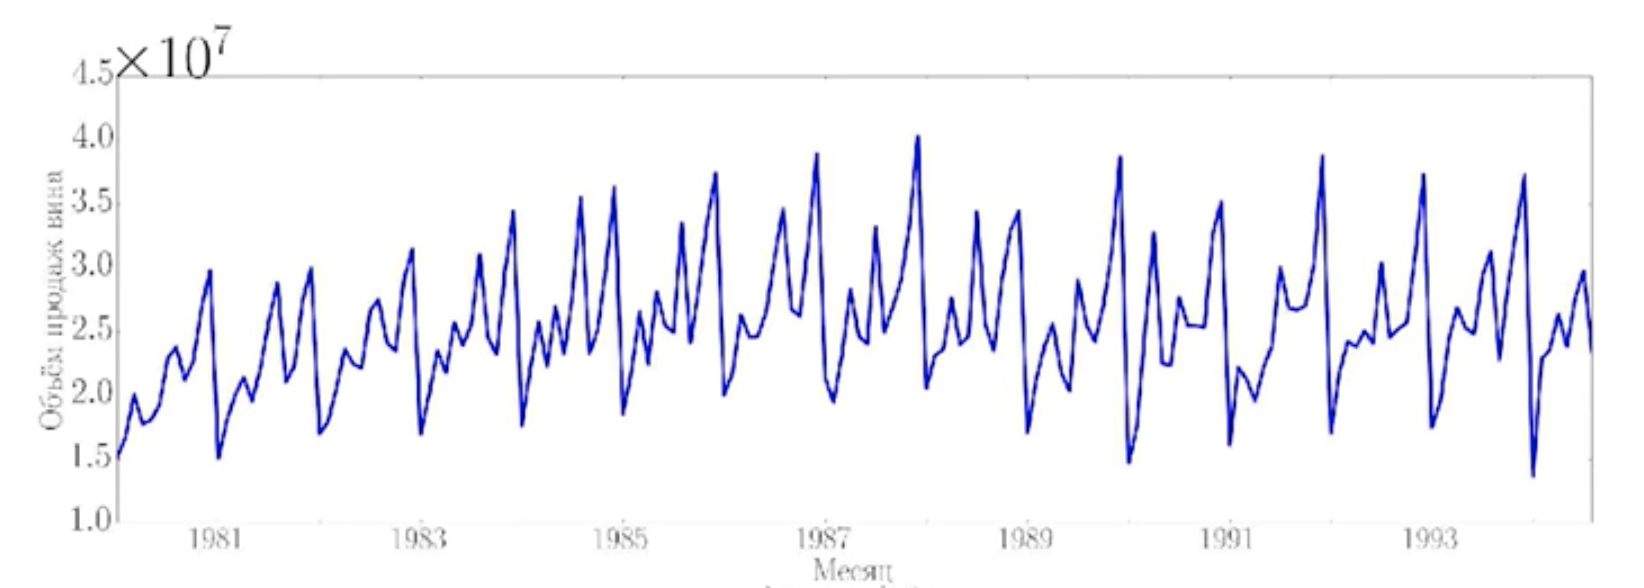
\includegraphics[totalheight=6cm]{autocorrelation/australian_vine.png}
	\caption{Временной ряд представляющий продажи вина в Австралии}
	\label{sec:autocorrelation:vine}
\end{figure}

На данном графике представлен временной ряд, показывающий объёмы продаж вина в Австралии. Как видно, на нём присутствует ярковыраженная сезонность, выпадающая на декабрь каждого года, сопоставленный с католическим рождеством.

На следующем графике будет представлена автокорреляционная функция для этого временного ряда \cite{datamining_in_action}.

\begin{figure}[h]
\centering
	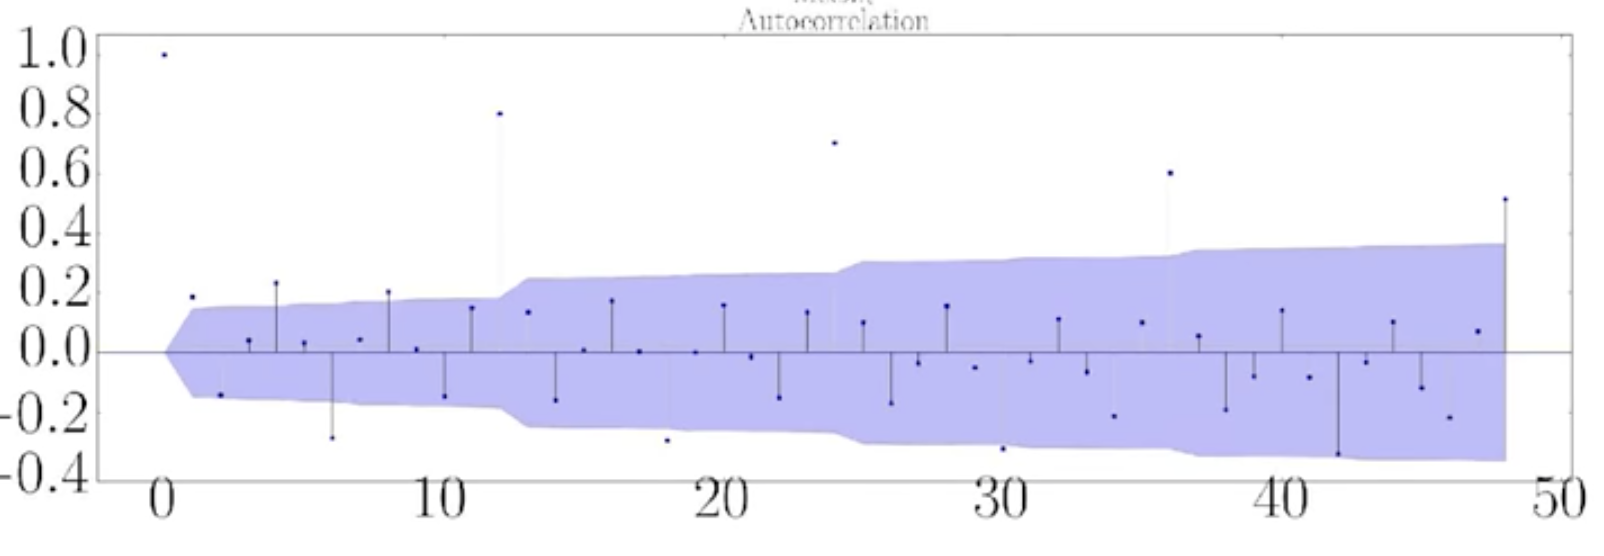
\includegraphics[totalheight=6cm]{autocorrelation/autocorrelation_vine.png}
	\caption{График автокорреляционной функции}
	\label{sec:autocorrelation:vine_auto}
\end{figure}

\textit{Автокорреляционная функция} - это график автокорреляции при разных значениях лага.

На рисунке \ref{sec:autocorrelation:vine_auto} каждый отрезок это значение автокорреляции. На графике видно, что есть пики на лагах кратных длине сезонного периода. Есть большая автокорреляция при значениях лага кратных 12 (12, 24, 36 и т.д.).

В ряде с контрактами сокровищницы США, рассмотренными ранее (\ref{sec:purpose:contracts}), если построить её график автокорреляционной функции можно увидеть следующую структуру \cite{datamining_in_action}:

\begin{figure}[h]
\centering
	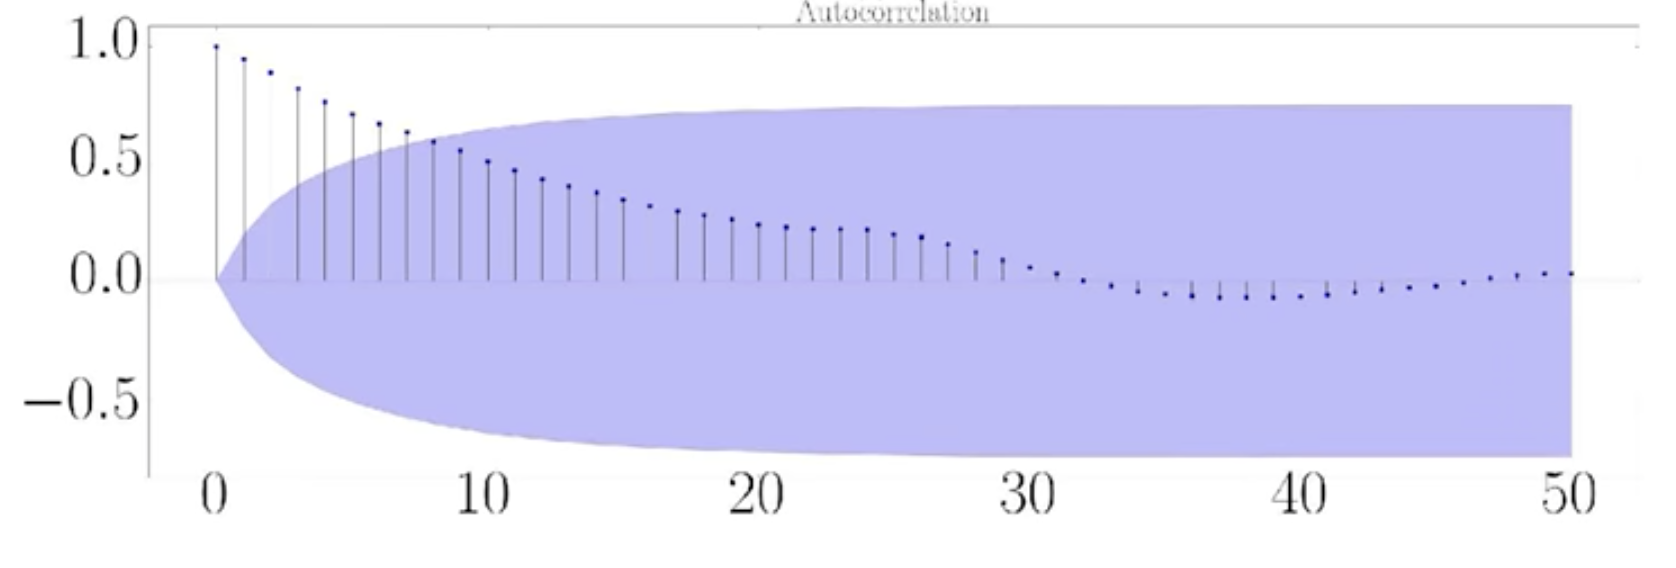
\includegraphics[totalheight=6cm]{autocorrelation/gold_autocorrelation.png}
	\caption{График автокорреляционной функции временного ряда количества контрактов сокровищницы США}
	\label{sec:autocorrelation:autocorrelation_usa_gold}
\end{figure}

Можно отметить, что типичная структура автокорреляции у которой <<сильный>> тренд, т.е. существует большая автокорреляция при малых лагах и она постепенно убывает и начинает синосуидально <<колебаться>> вокруг 0.

Стоит также рассмотреть график автокорреляции ранее описанного графика использования электричества в Австралии (\ref{sec:purpose:electricity}) \cite{datamining_in_action}.

\begin{figure}[h]
\centering
	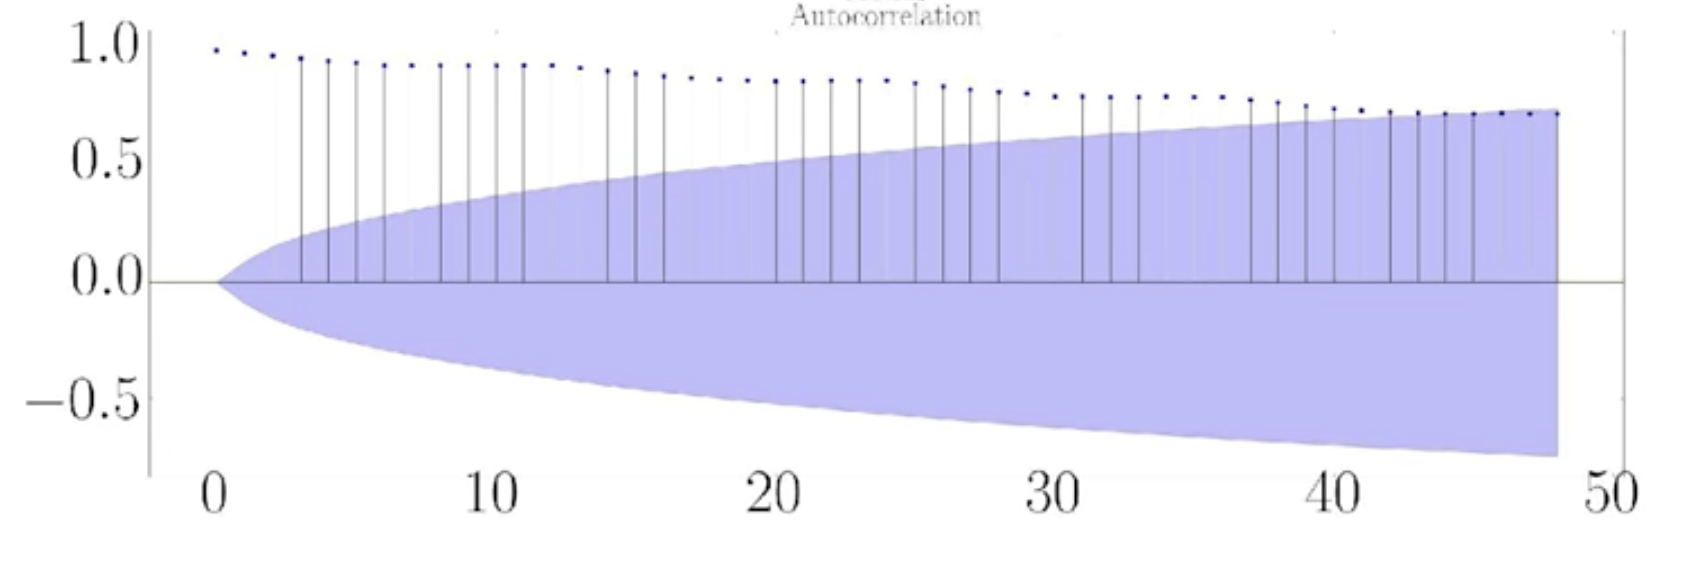
\includegraphics[totalheight=6cm]{autocorrelation/electricity_autocorrelation.png}
	\caption{График автокорреляционной функции временного ряда потребления электричества в Австралии}
	\label{sec:autocorrelation:autocorrelation_electricity}
\end{figure}

В этом ряде есть тренд и сезонность. Когда в ряде есть сезонность на лагах кратных сезонному периоду должны быть пики, однако, на данном графике их сложно разглядеть из за того, что в исходном ряде присутствует сильный тренд, который <<забивает>> общую картину.

Далее будет рассмотрен более сложный пример, на ранее рассмотренном ряде продажи жилых домов в США (\ref{sec:purpose:house-sells}) \cite{datamining_in_action}.

\begin{figure}[h]
\centering
	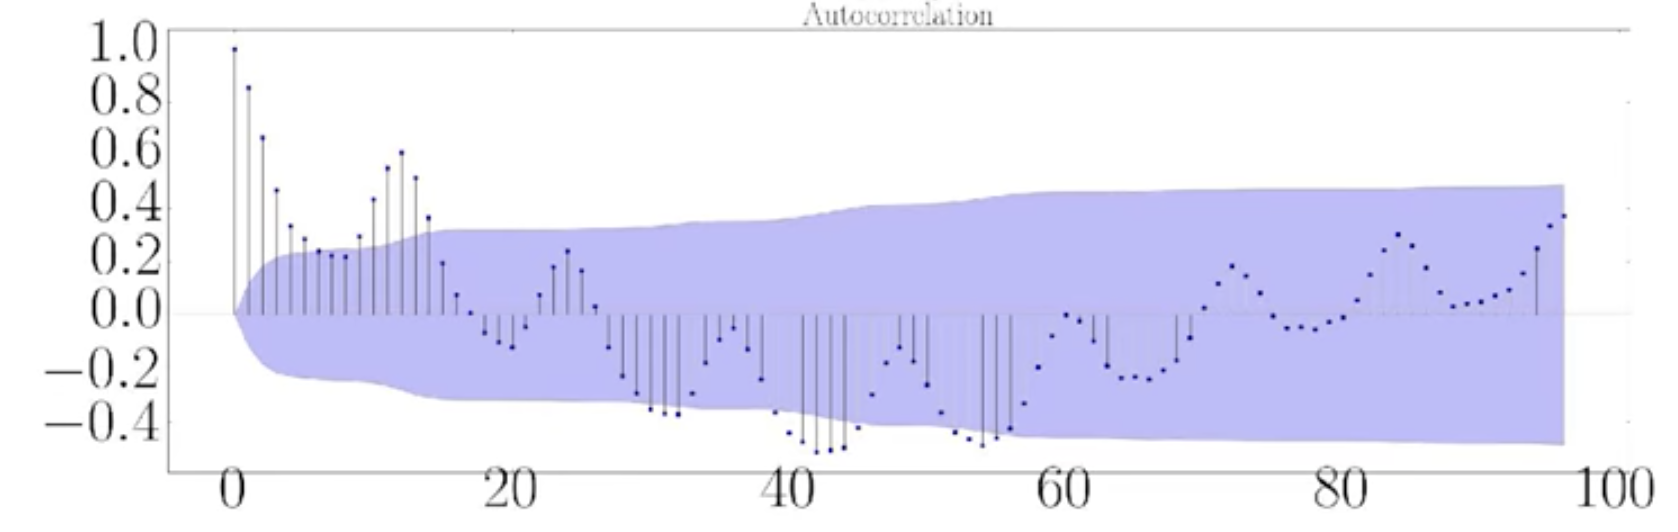
\includegraphics[totalheight=5cm]{autocorrelation/autocorrelation_houses.png}
	\caption{График автокорреляционной функции временного ряда продажи домов в США}
	\label{sec:autocorrelation:autocorrelation_electricity}
\end{figure}

На данном графике можно увидеть типичная автокорреляция для ряда, у которого присутствует сезонность и циклы. Циклы, в данном случае, приводят к тому, что постепенно происходит сдвиг местонахождения пика сезонного периода на некратное положение. В данном случае, первый пик находится на лаге равном 12, следующие не будет находится, в данном случае, не на 24. И так, постепенно происходит сдвиг пиков. Именно так циклы влияют на график автокорреляции - меняя положения пика сезонного периода.

И в заключение автокорреляционных графиков, стоит отметить график функции автокорреляции временного ряда с дневными значениями индекса Доу-Джонса \cite{datamining_in_action}.

\begin{figure}[h]
\centering
	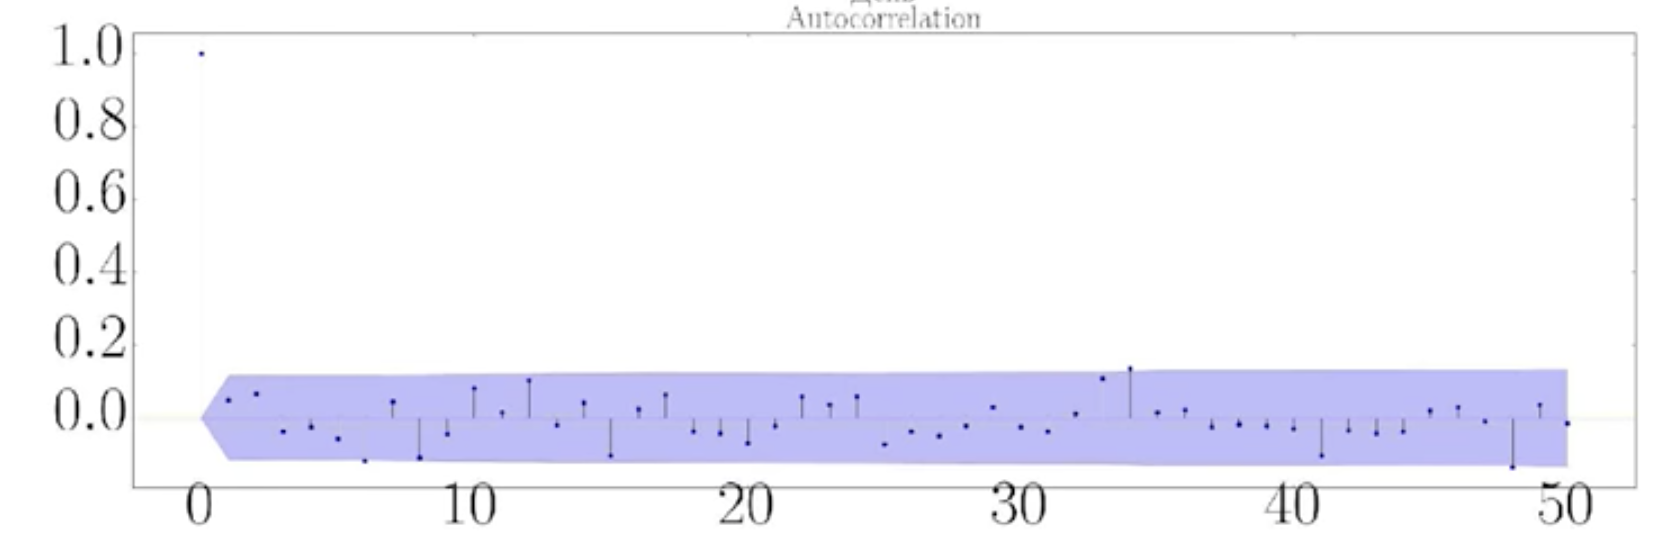
\includegraphics[totalheight=5cm]{autocorrelation/autocorrelation_dow_johnes.png}
	\caption{График автокорреляционной функции временного ряда значений индекса Доу-Джонса}
	\label{sec:autocorrelation:autocorrelation_dow_johnes}
\end{figure}

Данный график, показывает отсутствие какого либо наличия тренда, сезонов или циклов. В рассматриваемом примере, как и в любом примере, если даже сгенерировать для него шум, значения автокорреляционной функции будет в районе 0, что также можно отметить и на рисунке \ref{sec:autocorrelation:autocorrelation_dow_johnes}.

Значимость автокорреляции при каком-то фиксированном лаге можно проверить при помощи специальных критериев (например при помощи Q-критерия Льюинга-Бокса).